% Provenance (never printed): see sources/outline_sources.md (Year 2: radiogenic tracers
% Sr, Nd, Pb and mantle reservoirs; crustal growth; stable isotopes, delta notation and
% fractionation, d18O and d13C). Curves from figdata/bachelor-2/isotopes.py; exercise and
% problem values in the Book 4 scratch calculators calc/ch04.py and calc/ch04pb.py.
% Ruling (Sync 2): delta value and fractionation factor are chemistry's (Year 3 volume),
% recalled; this chapter defines the reference standards and the meteoric water line.
\chapter{Isotopengeochemie}\label{ch:b2:isotope-geochemistry}

Mangaia, in de zuidelijke Stille Oceaan, en Tristan da Cunha, in de zuidelijke
Atlantische Oceaan, zijn beide vulkanische eilanden van basalt, en een handstuk van
het ene lijkt sterk op een handstuk van het andere, of van een mid-oceanische rug.
Hun isotopen onderscheiden ze. Het strontium van de basalten van Mangaia draagt
hetzelfde aandeel strontium-87 als dat van de ruggen, ongeveer
$^{87}\mathrm{Sr}/^{86}\mathrm{Sr} = 0.7028$, terwijl hun lood tot het meest
radiogene op aarde behoort, met $^{206}\mathrm{Pb}/^{204}\mathrm{Pb}$ bij 21.6 tegen
18.4 voor de ruggen. De basalten van Tristan bevatten meer strontium-87, 0.7050 tot
0.7054, en minder neodymium-143 dan beide. Smelten sorteert de isotopen van
deze zware elementen niet, dus elke lava draagt de isotopensignatuur van de
mantel die smolt om haar te vormen: de aardmantel is niet één reservoir maar
meerdere, die miljarden jaren lang verschillende verhoudingen moeder--dochter hebben
behouden. Dit hoofdstuk gebruikt het radioactieve verval van rubidium, samarium, uranium
en thorium als een reeks tracers, volgt de evolutie van de mantel en de
continentale korst via de neodymiumisotopen, verdeelt de mantel in
reservoirs en mengsels van reservoirs, bespreekt hoe snel de continenten groeiden,
en eindigt met de lichte stabiele isotopen van zuurstof, waterstof en koolstof, die
de weg van water en koolstof door de aarde volgen.
% ledger: data:b4-oib-isotopes, gale13:isotopes

\begin{recall}
Een radioactieve moederkern vervalt met de snelheid $\lambda P$, en in een gesloten systeem
groeit de dochterverhouding als $(D/D_s)_{\text{nu}} = (D/D_s)_0 + (P/D_s)_{\text{nu}}
(e^{\lambda t}-1)$, waarbij $D_s$ een stabiele isotoop van de dochter is; mineralen of
gesteenten die samen zijn gevormd, liggen op een isochroon, waarvan de helling de ouderdom en het
snijpunt de beginverhouding geeft (Boek~2, laatste jaar; Boek~3,
hoofdstuk over radiometrische datering). Een massaspectrometer scheidt ionen naar hun
verhouding massa/lading (scheikunde, tweede jaar universiteit). De $\delta$-waarde van een
monster is $\delta = (R_{\text{monster}}/R_{\text{standaard}} - 1)\times 1000$, in
promille, en de fractioneringsfactor tussen twee fasen A en B is
$\alpha_{\mathrm{A/B}} = R_{\mathrm A}/R_{\mathrm B}$, waarbij $R$ de verhouding van de
zware tot de lichte isotoop is; beide worden, met de nulpuntsenergieën
die isotopenfractionering veroorzaken, ingevoerd in scheikunde, derde jaar universiteit.
\omterm{def:b2:elements-in-the-earth:partition}{Incompatibele elementen}, MORB en OIB werden gedefinieerd in
\cref{ch:b2:elements-in-the-earth}.
\end{recall}

\section{Radiogene isotopen als tracers}

Drie vervalsystemen dragen de meeste informatie over de mantel en de korst.
Rubidium-87 vervalt tot strontium-87, samarium-147 tot neodymium-143, en uranium
en thorium, via hun vervalreeksen, tot drie isotopen van lood. Moeder
en dochter gedragen zich telkens verschillend bij het smelten, en elke dochter heeft een
stabiele, niet-radiogene isotoop waartegen ze wordt gemeten.

\begin{table}[ht]
\centering
\begin{tabular}{lllll}
\hline
moeder & dochter & gemeten verhouding & vervalconstante (per jaar) & halveringstijd (Ga)\\
\hline
$^{87}$Rb & $^{87}$Sr & $^{87}\mathrm{Sr}/^{86}\mathrm{Sr}$ & \num{1.3972e-11} & 49.6\\
$^{147}$Sm & $^{143}$Nd & $^{143}\mathrm{Nd}/^{144}\mathrm{Nd}$ & \num{6.524e-12} & 106.25\\
$^{238}$U & $^{206}$Pb & $^{206}\mathrm{Pb}/^{204}\mathrm{Pb}$ & \num{1.55125e-10} & 4.47\\
\hline
\end{tabular}
\caption{Drie langlevende vervalsystemen die als tracers worden gebruikt. Gegevens: aanbevelingen
van IUPAC--IUGS (Villa en anderen, 2020 en 2022).}
\label{tab:b2:isotope-geochemistry:decay}
\end{table}
% ledger: villa22:rb87, villa20:sm147

\begin{definition}[Radiogene isotopentracer]\label{def:b2:isotope-geochemistry:tracer}
Een \emph{radiogene isotopentracer}\index{radiogene isotopentracer} is de verhouding
van een dochterisotoop, gevormd door een langlevende radioactieve moederkern, tot een stabiele
isotoop van hetzelfde element, zoals $^{87}\mathrm{Sr}/^{86}\mathrm{Sr}$ of
$^{143}\mathrm{Nd}/^{144}\mathrm{Nd}$, gebruikt om de bron van een gesteente te herkennen in plaats
van het te dateren. De verhouding van een reservoir groeit met een snelheid die bepaald wordt door zijn
verhouding moeder--dochter, en legt zo de geschiedenis van die verhouding vast.
\end{definition}

De twee elementen van een vervalpaar worden gescheiden telkens als de mantel smelt. In
\cref{ch:b2:elements-in-the-earth} bleek rubidium incompatibeler dan
strontium en neodymium incompatibeler dan samarium. Een smelt, en de korst
die ze opbouwt, verlaat de mantel daarom met een hoge Rb/Sr en een lage Sm/Nd; het
residu houdt een lage Rb/Sr en een hoge Sm/Nd. Na verloop van tijd wint de korst
sneller strontium-87 dan haar bron en trager neodymium-143; de \omterm{def:b2:isotope-geochemistry:reservoirs}{verarmde
mantel} doet het omgekeerde. De verhoudingen van de twee paren bewegen in tegengestelde
richtingen, wat het Sr--Nd-diagram hieronder duidelijk laat zien.

\begin{proposition}[Isotopenverhoudingen overleven het smelten]\label{prop:b2:isotope-geochemistry:melting}
Wanneer een gesteente smelt en de smelt zich van het residu scheidt, zijn de verhoudingen
$^{87}\mathrm{Sr}/^{86}\mathrm{Sr}$ en $^{143}\mathrm{Nd}/^{144}\mathrm{Nd}$ van
de smelt gelijk aan die van de bron, binnen de precisie van de
metingen; alleen de verhoudingen moeder--dochter, Rb/Sr en Sm/Nd, veranderen.
\end{proposition}
\admitted

\noindent De bewering berust op twee feiten. De isotopen van één element hebben
dezelfde elektronenstructuur, dus ze gaan bijna even gemakkelijk in een kristal of een smelt; het
relatieve massaverschil tussen strontium-87 en strontium-86, ongeveer één
procent, is veel kleiner dan voor zuurstof of waterstof, en bij hoge temperatuur daalt de
logaritme van een evenwichtsfractioneringsfactor met het omgekeerde kwadraat van
de temperatuur, naar 1. En de meting zelf corrigeert de
fractionering die in de massaspectrometer optreedt, door een verhouding van twee
niet-radiogene isotopen vast te leggen (voor neodymium $^{146}\mathrm{Nd}/^{144}\mathrm{Nd} =
0.7219$), wat ook elke kleine natuurlijke fractionering zou uitwissen. Een lava
bemonstert daarom de isotopenverhoudingen van haar bron, terwijl haar verhoudingen van
\omterm{def:b2:elements-in-the-earth:trace}{sporenelementen} ook het smelten weerspiegelen.
% ledger: white:chur, white:t-dependence

\section{De evolutie van mantel en korst}

\subsection{Het chondritische reservoir}

Samarium en neodymium zijn beide refractaire lithofiele \omterm{def:b2:elements-in-the-earth:ree}{zeldzame aarden}
(\cref{ch:b2:elements-in-the-earth}): de \omterm{def:b2:elements-in-the-earth:bse}{totale silicaataarde} zou hun
chondritische verhouding moeten hebben behouden. De \omterm{def:b2:planet-formation-meteorites:chondrule}{chondrieten} geven dan de Sm--Nd-geschiedenis van de
ongedifferentieerde aarde.

\begin{definition}[Chondritisch uniform reservoir]\label{def:b2:isotope-geochemistry:chur}
Het \emph{chondritisch uniform reservoir}\index{chondritisch uniform reservoir}
(CHUR) is een modelreservoir met de samarium--neodymiumsamenstelling van de
\omterm{def:b2:planet-formation-meteorites:chondrule}{chondrieten}, gesloten sinds de vorming van het zonnestelsel. Zijn huidige
verhoudingen zijn $(^{143}\mathrm{Nd}/^{144}\mathrm{Nd})_{\mathrm{CHUR}} = 0.512638$ en
$(^{147}\mathrm{Sm}/^{144}\mathrm{Nd})_{\mathrm{CHUR}} = 0.1966$.
\end{definition}
% ledger: white:chur

Terugberekend met de isochroonvergelijking had CHUR, toen de eerste vaste stoffen
\qty{4567}{Myr} geleden condenseerden (\cref{ch:b2:planet-formation-meteorites}),
\[
  ^{143}\mathrm{Nd}/^{144}\mathrm{Nd} = 0.512638 - 0.1966\,\bigl(e^{\lambda\cdot
  \num{4.567e9}\,\mathrm{yr}}-1\bigr) = 0.506692 .
\] Sindsdien is zijn verhouding gegroeid met
1.2 procent. De verschillen tussen aardse gesteenten zijn duizend keer
kleiner en worden in een handiger eenheid opgegeven.
% ledger: lugaro:cai, villa20:sm147

\begin{definition}[Epsilonnotatie]\label{def:b2:isotope-geochemistry:epsilon}
De \emph{epsilonnotatie}\index{epsilonnotatie} drukt de verhouding
$^{143}\mathrm{Nd}/^{144}\mathrm{Nd}$ van een monster, op een tijdstip $t$ vóór het
heden, uit als haar relatieve afwijking van CHUR op hetzelfde tijdstip, in delen per
tienduizend:
\[
  \varepsilon_{\mathrm{Nd}}(t) = \left(
  \frac{(^{143}\mathrm{Nd}/^{144}\mathrm{Nd})_{\text{monster}}(t)}
       {(^{143}\mathrm{Nd}/^{144}\mathrm{Nd})_{\mathrm{CHUR}}(t)} - 1\right)\times 10^4 .
\]
Zonder tijdstip is $\varepsilon_{\mathrm{Nd}}$ de huidige waarde.
\end{definition}

De gemiddelde MORB, met $^{143}\mathrm{Nd}/^{144}\mathrm{Nd} = 0.513074$, heeft
$\varepsilon_{\mathrm{Nd}} = (0.513074/0.512638 - 1)\times10^4 = +8.5$; de meeste gesteenten
liggen tussen $-20$ en $+10$. Een positieve waarde betekent dat de bron van het gesteente
gemiddeld over de geschiedenis van de aarde een hogere Sm/Nd heeft gehad dan de
\omterm{def:b2:planet-formation-meteorites:chondrule}{chondrieten}: ze is verarmd in het incompatibelere element, neodymium. Een
negatieve waarde betekent het omgekeerde. De afwijking van de chondritische Sm/Nd wordt gemeten met de
relatieve afwijking
\[
  f_{\mathrm{Sm/Nd}} = \frac{(\mathrm{Sm}/\mathrm{Nd})_{\text{monster}}}
  {(\mathrm{Sm}/\mathrm{Nd})_{\mathrm{CHUR}}} - 1,
\]
die dezelfde is, of de verhoudingen nu in massa of in atomen zijn. Met de CI-waarden
van \cref{ch:b2:elements-in-the-earth} (Sm 0.145, Nd \qty{0.457}{ppm},
$\mathrm{Sm}/\mathrm{Nd} = 0.317$) heeft de bovenste continentale korst (4.7 en
\qty{27}{ppm}, 0.174) $f_{\mathrm{Sm/Nd}} = -0.45$.
% ledger: gale13:isotopes, white:chur, lodders:ci-table, rg03:ucc-trace

\begin{proposition}[Lineaire groei van $\varepsilon_{\mathrm{Nd}}$]\label{prop:b2:isotope-geochemistry:linear}
Een reservoir dat zich van CHUR heeft afgesplitst en sindsdien de relatieve afwijking
$f_{\mathrm{Sm/Nd}}$ heeft behouden, verandert zijn $\varepsilon_{\mathrm{Nd}}$, vooruit in
de tijd, met de snelheid
\[
  \frac{\mathrm{d}\varepsilon_{\mathrm{Nd}}}{\mathrm{d}\tau} \approx Q\,f_{\mathrm{Sm/Nd}},
  \qquad
  Q = 10^4\,\lambda_{147}\,
  \frac{(^{147}\mathrm{Sm}/^{144}\mathrm{Nd})_{\mathrm{CHUR}}}
       {(^{143}\mathrm{Nd}/^{144}\mathrm{Nd})_{\mathrm{CHUR}}}
  = \qty{25.0}{\per\giga\year},
\]
waarbij $\tau$ de vooruit getelde tijd is. Een reservoir met $\varepsilon_0$ bij zijn
afsplitsing, een tijd $T$ geleden, heeft vandaag $\varepsilon_{\mathrm{Nd}} \approx \varepsilon_0
+ Q f_{\mathrm{Sm/Nd}} T$.
\end{proposition}

\begin{proof}
Schrijf $R$ voor $^{143}\mathrm{Nd}/^{144}\mathrm{Nd}$ en $p$ voor
$^{147}\mathrm{Sm}/^{144}\mathrm{Nd}$. In een gesloten reservoir geldt
$\mathrm{d}R/\mathrm{d}\tau = \lambda p\,e^{\lambda t}$, met $t$ de tijd vóór het
heden; omdat $\lambda t \le 0.03$, verschilt de factor $e^{\lambda t}$ hoogstens
3 procent van 1, en $\mathrm{d}R/\mathrm{d}\tau \approx \lambda p$. Dan
$\mathrm{d}(R_s - R_c)/\mathrm{d}\tau \approx \lambda (p_s - p_c) = \lambda p_c
f_{\mathrm{Sm/Nd}}$, want $p_s/p_c - 1 = f_{\mathrm{Sm/Nd}}$. Delen door $R_c$,
dat over de ouderdom van de aarde maar 1.2 procent verandert, geeft
$\mathrm{d}\varepsilon/\mathrm{d}\tau \approx 10^4\lambda p_c f/R_c$. Met
$\lambda = \qty{6.524e-12}{\per\year}$, $p_c = 0.1966$ en $R_c = 0.512638$ is $Q =
\num{2.502e-8}$ per jaar, \qty{25.0}{\per\giga\year}.
\end{proof}
% ledger: villa20:sm147, white:chur

Een korst met de Sm/Nd van de bovenste korst ($f = -0.45$) verliest daarom ongeveer
11 epsiloneenheden per miljard jaar ten opzichte van CHUR, terwijl een mantelreservoir
maar $f = +0.07$ nodig heeft om in \qty{4.567}{Ga} van 0 tot de MORB-waarde van $+8.5$
te stijgen. De figuur hieronder volgt de exacte vergelijkingen voor drie
reservoirs: CHUR, een \omterm{def:b2:isotope-geochemistry:reservoirs}{verarmde mantel} die gesloten is sinds de vorming van de aarde, met de Sm/Nd
die hem vandaag op de MORB-waarde brengt ($^{147}\mathrm{Sm}/^{144}\mathrm{Nd} =
0.211$), en een korst die 2.7 miljard jaar geleden aan die mantel is onttrokken, met de
Sm/Nd van de bovenste korst ($0.108$). De korst begon bij $\varepsilon_{\mathrm{Nd}} =
+3.5$, de waarde van haar bron op dat moment, en staat nu op $-27$.

\begin{definition}[Verarmde mantel, verrijkte mantel]\label{def:b2:isotope-geochemistry:reservoirs}
Een \emph{verarmde mantel}\index{verarmde mantel} is een deel van de mantel dat
\omterm{def:b2:elements-in-the-earth:partition}{incompatibele elementen} aan smelten heeft afgestaan, zodat zijn Sm/Nd hoger en zijn Rb/Sr
lager is dan chondritisch; met de tijd wordt zijn $\varepsilon_{\mathrm{Nd}}$ positief en
zijn $^{87}\mathrm{Sr}/^{86}\mathrm{Sr}$ laag. Een \emph{verrijkte
mantel}\index{verrijkte mantel} is een deel van de mantel dat
\omterm{def:b2:elements-in-the-earth:partition}{incompatibele elementen} heeft gewonnen, bijvoorbeeld uit gerecyclede korst of uit kleine smelten,
met een negatieve $\varepsilon_{\mathrm{Nd}}$ of een hoge $^{87}\mathrm{Sr}/^{86}\mathrm{Sr}$.
\end{definition}

\begin{omfigure}
\centering
\begin{tikzpicture}
\begin{axis}[omrecord, width=0.82\linewidth, height=6.4cm,
  x dir=reverse, xmin=0, xmax=4.6, ymin=-30, ymax=12,
  xlabel={tijd vóór het heden (Ga)}, ylabel={$\varepsilon_{\mathrm{Nd}}(t)$},
  tick label style={font=\scriptsize}, label style={font=\small}]
\addplot[thick, black] table[x=t_Ga, y=eps] {figdata/out/bachelor-2-isotopes-chur.dat};
\addplot[very thick, blue!70!black] table[x=t_Ga, y=eps] {figdata/out/bachelor-2-isotopes-dm.dat};
\addplot[very thick, brown!70!black] table[x=t_Ga, y=eps] {figdata/out/bachelor-2-isotopes-crust.dat};
\addplot[densely dashed, gray] coordinates {(2.7,-30) (2.7,12)};
\node[font=\scriptsize, anchor=north] at (axis cs:3.6,-0.6) {CHUR};
\node[font=\scriptsize, blue!70!black, anchor=south east] at (axis cs:0.4,8.8) {verarmde mantel, $+8.5$};
\node[font=\scriptsize, brown!70!black, anchor=north east] at (axis cs:0.3,-25.5) {korst, $-27$};
\node[font=\scriptsize, gray, anchor=north west, align=left] at (axis cs:2.65,-12) {korst onttrokken\\op \qty{2.7}{Ga}};
\end{axis}
\end{tikzpicture}
\par\smallskip{\small Evolutie van de neodymiumisotopen, als $\varepsilon_{\mathrm{Nd}}$, van
het chondritische reservoir (per definitie nul), van een \omterm{def:b2:isotope-geochemistry:reservoirs}{verarmde mantel} die gesloten is sinds
\qty{4.567}{Ga} en waarvan de Sm/Nd hem vandaag op de gemiddelde MORB brengt, en van een korst
die er \qty{2.7}{Ga} geleden aan is onttrokken met de Sm/Nd van de bovenste continentale
korst. Elke lijn is bijna recht, zoals de propositie over lineaire groei zegt. Gegevens:
CHUR, het leerboek van White; gemiddelde MORB, Gale en anderen (2013); Sm/Nd van de korst,
Rudnick en Gao.}
\end{omfigure}
% ledger: white:chur, villa20:sm147, gale13:isotopes, rg03:ucc-trace, lodders:ci-table, lugaro:cai

\subsection{Twee complementaire reservoirs}

Als de continentale korst en de \omterm{def:b2:isotope-geochemistry:reservoirs}{verarmde mantel} uit één chondritisch
reservoir zijn gemaakt, moet hun neodymium samen weer de chondritische waarde geven. Neodymium is
de drager: elk reservoir telt mee in verhouding tot het neodymium dat het bevat.

\begin{proposition}[Isotopische massabalans]\label{prop:b2:isotope-geochemistry:mass-balance}
Laat reservoirs $i$ met massa's $M_i$ en neodymiumconcentraties $C_i$ voortkomen uit
de opsplitsing van één moederreservoir. Dan geldt, in zeer goede benadering,
\[
  \sum_i M_i C_i\, \varepsilon_i = \Bigl(\sum_i M_i C_i\Bigr) \varepsilon_{\text{moeder}},
\]
waarbij beide leden op hetzelfde tijdstip worden geëvalueerd, en het moederreservoir wordt gevolgd alsof
het heel was gebleven.
\end{proposition}

\begin{proof}
Het aantal $^{143}\mathrm{Nd}$-atomen en het aantal $^{144}\mathrm{Nd}$-atomen
blijven elk behouden bij de opsplitsing, en elk groeit later (voor
$^{143}\mathrm{Nd}$) of blijft gelijk (voor $^{144}\mathrm{Nd}$) in elk reservoir precies zoals
in het geheel. Het met $^{144}\mathrm{Nd}$ gewogen gemiddelde van de verhoudingen $R_i$ is dus gelijk aan
de verhouding van het moederreservoir, $R_p$. Het aandeel van $^{144}\mathrm{Nd}$ in neodymium verschilt
tussen reservoirs veel minder dan één op duizend, dus wegen met
$M_iC_i$ is hetzelfde als wegen met $^{144}\mathrm{Nd}$. Ten slotte is $\varepsilon$ een
lineaire functie van $R$ op een gegeven tijdstip, $\varepsilon = 10^4(R/R_c - 1)$, en een
gewogen gemiddelde van lineaire functies is de lineaire functie van het gewogen gemiddelde.
\end{proof}

Als de waarde van de bovenste korst, \qty{27}{ppm} neodymium, voor de hele
korst wordt genomen, bevat een continentale korst van \qty{7.2e9}{km^3} bij \qty{2830}{kg/m^3}, dat is
\qty{2.0e22}{kg} of 0.51 procent van de massa van de silicaataarde,
$0.0051\times27/1.25 = 11$ procent van het neodymium van de silicaataarde (\omterm{def:b2:elements-in-the-earth:bse}{primitieve
mantel}, \qty{1.25}{ppm}). Als de korst een gemiddelde $\varepsilon_{\mathrm{Nd}}$ van
$-15$ heeft, moet een negatieve bijdrage van $0.11\times15 = 1.65$ eenheden
door de mantel worden gecompenseerd: een reservoir met de MORB-waarde van $+8.5$ zou
ongeveer een vijfde van het neodymium van de silicaataarde moeten bevatten (\cref{exo:b2:isotope-geochemistry:9}). Dit is een van de
argumenten dat de \omterm{def:b2:isotope-geochemistry:reservoirs}{verarmde mantel} die de ruggen bemonsteren niet de hele
mantel is.
% ledger: cogley84:continents, cm95:crust, ms95:pm-trace, rg03:ucc-trace, data:prem, earth:mass, gale13:isotopes

\section{De reservoirs van de mantel}

De isotopenverhoudingen van oceanische basalten bemonsteren de mantel zonder door
de continentale korst te gaan. Tegen elkaar uitgezet tonen ze zowel de
complementariteit van korst en \omterm{def:b2:isotope-geochemistry:reservoirs}{verarmde mantel} als het bestaan van andere
reservoirs.

Strontium- en neodymiumisotopen zijn in de meeste oceanische basalten anticorreleerd: een
lava met een hoge $\varepsilon_{\mathrm{Nd}}$ heeft een lage
$^{87}\mathrm{Sr}/^{86}\mathrm{Sr}$. Deze band heet de mantelreeks; hij volgt
uit het tegengestelde gedrag van de twee paren bij het smelten (rubidium minder
compatibel dan strontium, samarium compatibeler dan neodymium). De gemiddelde
MORB ligt aan het verarmde uiteinde, met $^{87}\mathrm{Sr}/^{86}\mathrm{Sr} = 0.702819$ en
$\varepsilon_{\mathrm{Nd}} = +8.5$. \omterm{def:b2:elements-in-the-earth:morb-oib}{Oceaaneilandbasalten} spreiden zich van daaruit naar
lagere $\varepsilon_{\mathrm{Nd}}$ en hogere $^{87}\mathrm{Sr}/^{86}\mathrm{Sr}$, maar niet
langs één enkele lijn.
% ledger: white:dm, gale13:isotopes

\begin{definition}[Eindlid van de mantel]\label{def:b2:isotope-geochemistry:end-members}
Een \emph{eindlid van de mantel}\index{eindlid van de mantel} is een van de extreme
isotopensamenstellingen waaruit de isotopenverhoudingen van Sr, Nd en Pb van oceanische
basalten door menging kunnen worden opgebouwd. Vier worden gewoonlijk benoemd: DMM, de verarmde
MORB-mantel (lage $^{87}\mathrm{Sr}/^{86}\mathrm{Sr}$, hoge $\varepsilon_{\mathrm{Nd}}$);
HIMU, naar een hoge $\mu = {}^{238}\mathrm{U}/^{204}\mathrm{Pb}$ in zijn bron
(zeer radiogeen lood, $^{206}\mathrm{Pb}/^{204}\mathrm{Pb}$ boven 20, met lage
$^{87}\mathrm{Sr}/^{86}\mathrm{Sr}$); EM1, \omterm{def:b2:isotope-geochemistry:reservoirs}{verrijkte mantel} 1 (matig hoge
$^{87}\mathrm{Sr}/^{86}\mathrm{Sr}$, negatieve $\varepsilon_{\mathrm{Nd}}$, weinig radiogeen
lood); en EM2, \omterm{def:b2:isotope-geochemistry:reservoirs}{verrijkte mantel} 2 (hoge $^{87}\mathrm{Sr}/^{86}\mathrm{Sr}$).
\end{definition}
% ledger: white:end-members

\begin{omfigure}
\centering
\begin{tikzpicture}
\begin{axis}[omrecord, width=0.82\linewidth, height=6.6cm,
  xmin=0.7020, xmax=0.7064, ymin=-6, ymax=11,
  xlabel={$^{87}\mathrm{Sr}/^{86}\mathrm{Sr}$}, ylabel={$\varepsilon_{\mathrm{Nd}}$},
  xticklabel style={/pgf/number format/fixed, /pgf/number format/precision=4},
  scaled x ticks=false, legend pos=south west, legend cell align=left,
  legend style={font=\scriptsize}, tick label style={font=\scriptsize},
  label style={font=\small}]
\addplot[only marks, mark=*, mark size=1.3pt, red!70!black] table[x=sr, y=eps] {figdata/out/bachelor-2-isotopes-himu.dat};
\addlegendentry{HIMU-type: St.\ Helena, Mangaia, Tubuai}
\addplot[only marks, mark=square*, mark size=1.2pt, brown!70!black] table[x=sr, y=eps] {figdata/out/bachelor-2-isotopes-em1.dat};
\addlegendentry{EM1-type: Tristan da Cunha, Gough}
\addplot[only marks, mark=diamond*, mark size=3pt, blue!70!black] table[x=sr, y=eps] {figdata/out/bachelor-2-isotopes-morb.dat};
\addlegendentry{gemiddelde MORB}
\addplot[densely dashed, gray] coordinates {(0.7020,0) (0.7064,0)};
\node[font=\scriptsize, gray, anchor=south east] at (axis cs:0.7063,0.1) {CHUR};
\draw[->, gray] (axis cs:0.7030,9.5) -- (axis cs:0.7046,0.8);
\node[font=\scriptsize, gray, anchor=west, align=left] at (axis cs:0.7036,6.5) {de mantelreeks:\\verarmd tot verrijkt};
\end{axis}
\end{tikzpicture}
\par\smallskip{\small Strontium- en neodymiumisotopen van 89 basalten van vijf
oceaaneilanden en van het gemiddelde \omterm{def:b2:elements-in-the-earth:morb-oib}{basalt van mid-oceanische ruggen}. De eilanden van het HIMU-type liggen
onder de hoofdreeks, met de lage strontiumverhouding van MORB maar een lagere
$\varepsilon_{\mathrm{Nd}}$; de eilanden van het EM1-type liggen aan de verrijkte kant van CHUR.
Samoaanse lava's van het EM2-type bereiken $^{87}\mathrm{Sr}/^{86}\mathrm{Sr} = 0.7205$, ver
rechts buiten deze schaal. Gegevens: Stracke en anderen (2022), CC BY 4.0; Gale en
anderen (2013); Edwards en anderen (2019).}
\end{omfigure}
% ledger: data:b4-oib-isotopes, gale13:isotopes, edwards19:samoa, white:chur

De eilandgroepen van de figuur hierboven zijn niet willekeurig. De St.-Helenagroep,
die de Australeilanden (waaronder Mangaia en Tubuai) en
Ascension omvat, ligt onder de hoofdreeks en heeft het meest radiogene lood
($^{206}\mathrm{Pb}/^{204}\mathrm{Pb}$ boven 20; Mangaia bereikt 21.5 tot 22.0). De
Kerguelengroep, Tristan da Cunha, Gough en Kerguelen, ligt bij matig hoge
$^{87}\mathrm{Sr}/^{86}\mathrm{Sr}$ en negatieve $\varepsilon_{\mathrm{Nd}}$, altijd met
weinig radiogeen lood. De Genootschapsgroep, met Samoa en de Marquesaseilanden, bepaalt een
vlakkere Sr--Nd-trend die zeer hoge strontiumverhoudingen bereikt: twee Samoaanse lava's
hebben een $^{87}\mathrm{Sr}/^{86}\mathrm{Sr}$ van 0.7186 en 0.7205, hoger dan het huidige
zeewater (0.7092). De St.-Helena-, Kerguelen- en Genootschapsgroep zijn de typen HIMU,
EM1 en EM2.
% ledger: white:end-members, data:b4-oib-isotopes, edwards19:samoa

Een verhouding die tussen twee delen van de mantel verschilt, moet lange tijd door een
verschil in verhouding moeder--dochter in stand zijn gehouden: een
verschil van 10 eenheden $\varepsilon_{\mathrm{Nd}}$ vraagt volgens de propositie over
lineaire groei 1 miljard jaar bij $f = 0.4$ of 4 miljard jaar bij $f = 0.1$. De
mantelreservoirs zijn daarom oud. Wat ze zijn, volgt uit de
verhoudingen moeder--dochter die hun isotopen vereisen. HIMU vraagt lange tijd een hoge U/Pb en een lage
Rb/Sr, wat past bij oceanische korst die lood en rubidium verloor
in de fluïda die boven een subductiezone vrijkomen, en die daarna één of twee miljard jaar in de mantel
werd opgeslagen. EM1 en EM2 vragen een lage Sm/Nd en, voor EM2, een hoge
Rb/Sr: het kenmerk van materiaal dat van de continenten afkomstig is, zoals gerecycled
sediment, of van mantel die door kleine smelten is verrijkt. Deze interpretaties staan
ter discussie; de metingen niet.
% ledger: white:end-members

\begin{omfigure}
\centering
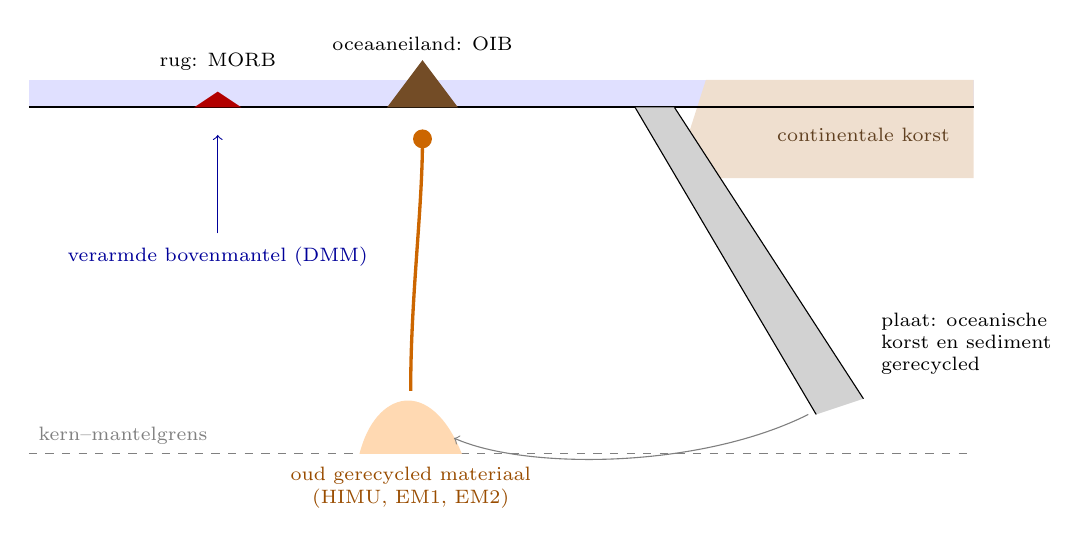
\begin{tikzpicture}[x=1cm, y=1cm, font=\scriptsize]
  % surface and lithosphere
  \fill[blue!12] (-6,0) rectangle (6,0.35);
  \fill[brown!25] (2.6,0.35) -- (6,0.35) -- (6,-0.9) -- (2.2,-0.9) -- cycle;
  \node[brown!50!black] at (4.6,-0.35) {continentale korst};
  \draw[thick] (-6,0) -- (6,0);
  % ridge
  \node[anchor=south] at (-3.6,0.35) {rug: MORB};
  \draw[->, blue!60!black] (-3.6,-1.6) -- (-3.6,-0.35);
  \node[blue!60!black, anchor=north] at (-3.6,-1.65) {verarmde bovenmantel (DMM)};
  % slab
  \fill[gray!35] (1.7,0) -- (2.2,0) -- (4.6,-3.7) -- (4.0,-3.9) -- cycle;
  \draw (1.7,0) -- (4.0,-3.9) (2.2,0) -- (4.6,-3.7);
  \node[anchor=west, align=left] at (4.7,-3.0) {plaat: oceanische\\korst en sediment\\gerecycled};
  % deep pool and plume
  \draw[gray, dashed] (-6,-4.4) -- (6,-4.4);
  \node[anchor=south west, gray] at (-6,-4.4) {kern--mantelgrens};
  \fill[orange!30] (-1.8,-4.4) .. controls (-1.6,-3.6) and (-0.9,-3.4) .. (-0.5,-4.4) -- cycle;
  \draw[very thick, orange!80!black] (-1.15,-3.6) .. controls (-1.15,-2.4) and (-1.0,-1.3) .. (-1.0,-0.4);
  \fill[orange!80!black] (-1.0,-0.4) circle (0.12);
  \fill[brown!60!black] (-1.45,0) -- (-1.0,0.6) -- (-0.55,0) -- cycle;
  \node[anchor=south] at (-1.0,0.6) {oceaaneiland: OIB};
  \fill[red!70!black] (-3.9,0) -- (-3.6,0.2) -- (-3.3,0) -- cycle;
  \node[orange!60!black, anchor=north, align=center] at (-1.15,-4.45) {oud gerecycled materiaal\\(HIMU, EM1, EM2)};
  \draw[->, gray] (3.9,-3.9) .. controls (2.5,-4.6) and (0.3,-4.6) .. (-0.6,-4.2);
\end{tikzpicture}
\par\smallskip{\small Een veelgebruikte interpretatie van de mantelreservoirs, niet op
schaal: de ruggen bemonsteren de verarmde bovenmantel; oceanische korst en sediment
keren bij subductiezones naar de mantel terug; pluimen die uit de diepe mantel opstijgen,
brengen materiaal omhoog waarin oude gerecyclede componenten zijn gemengd, en geven de
eilanden hun HIMU-, EM1- of EM2-karakter.}
\end{omfigure}

\section{Menging}

Veel isotopenreeksen zijn mengsels. Een lava kan uit een bron komen die een
mengsel van twee reservoirs is, of een magma kan wat van de korst opnemen die het doorkruist.
Beide gevallen volgen dezelfde algebra.

\begin{proposition}[Menghyperbool]\label{prop:b2:isotope-geochemistry:mixing}
Laat een mengsel een massafractie $f$ van component A en $1-f$ van component
B bevatten. Voor een element met concentraties $C_{\mathrm A}$, $C_{\mathrm B}$ en isotopenverhoudingen
$R_{\mathrm A}$, $R_{\mathrm B}$ geldt:
\begin{enumerate}
\item de concentratie van het mengsel, $C = fC_{\mathrm A} + (1-f)C_{\mathrm B}$, en
haar isotopenverhouding,
$R = \bigl(fC_{\mathrm A}R_{\mathrm A} + (1-f)C_{\mathrm B}R_{\mathrm B}\bigr)/C$, voldoen aan
$R = a + b/C$ met constanten $a$ en $b$: de mengsels liggen op een rechte lijn in
een diagram van $R$ tegen $1/C$;
\item twee zulke verhoudingen van twee elementen, $R$ en $R'$, liggen op een hyperbool, de
\emph{menghyperbool}\index{menghyperbool}, die alleen een rechte lijn is
als de verhouding van de twee elementen in A en B dezelfde is. Haar kromming wordt bepaald door
$K = (C'/C)_{\mathrm A}/(C'/C)_{\mathrm B}$.
\end{enumerate}
\end{proposition}

\begin{proof}
(1) Elimineer $f$: $f = (C - C_{\mathrm B})/(C_{\mathrm A} - C_{\mathrm B})$. Dan is
$RC = C_{\mathrm B}R_{\mathrm B} + f(C_{\mathrm A}R_{\mathrm A} - C_{\mathrm B}R_{\mathrm
B})$ lineair in $C$, $RC = \alpha + \beta C$, en $R = \beta + \alpha/C$.
(2) Het aandeel van het element dat van A komt, is $s = fC_{\mathrm A}/C$, en $R =
R_{\mathrm B} + s(R_{\mathrm A} - R_{\mathrm B})$ is lineair in $s$; evenzo is $R'$
lineair in $s' = fC'_{\mathrm A}/C'$. Met $u = f/(1-f)$ is $s = u C_{\mathrm
A}/(uC_{\mathrm A} + C_{\mathrm B})$ en $s' = uC'_{\mathrm A}/(uC'_{\mathrm A} +
C'_{\mathrm B})$. Eliminatie van $u$ geeft $s' = Ks/(1 + (K-1)s)$, een hyperbool in het
$(s, s')$-vlak, dus in het $(R, R')$-vlak; het is de rechte $s' = s$
als $K = 1$.
\end{proof}

\begin{omfigure}
\centering
\begin{tikzpicture}
\begin{axis}[omrecord, width=0.62\linewidth, height=6.2cm,
  xmin=0, xmax=1, ymin=0, ymax=1,
  xlabel={eerste verhouding, herschaald (B $=0$, A $=1$)},
  ylabel={tweede verhouding, herschaald},
  tick label style={font=\scriptsize}, label style={font=\small}]
\addplot[thick, red!70!black] table[x=x, y=y] {figdata/out/bachelor-2-isotopes-mixK50.dat};
\addplot[thick, black] table[x=x, y=y] {figdata/out/bachelor-2-isotopes-mixK10.dat};
\addplot[thick, blue!70!black] table[x=x, y=y] {figdata/out/bachelor-2-isotopes-mixK02.dat};
\node[font=\scriptsize, red!70!black, anchor=south east] at (axis cs:0.30,0.72) {$K=5$};
\node[font=\scriptsize, anchor=south east] at (axis cs:0.55,0.56) {$K=1$};
\node[font=\scriptsize, blue!70!black, anchor=north west] at (axis cs:0.62,0.22) {$K=0.2$};
\node[font=\scriptsize, anchor=north west] at (axis cs:0.0,0.0) {B};
\node[font=\scriptsize, anchor=south east] at (axis cs:1.0,1.0) {A};
\end{axis}
\end{tikzpicture}
\par\smallskip{\small Mengkrommen tussen twee componenten A en B voor drie
waarden van $K$, de verhouding van de twee elementen in A gedeeld door die in B. Elke
isotopenverhouding is herschaald naar 0 bij B en 1 bij A; het tweede element is $K$ keer
rijker in A, ten opzichte van het eerste, dan in B, dus de tweede verhouding beweegt sneller naar
A toe als $K > 1$.}
\end{omfigure}

Een component die rijk is aan een element, overheerst de isotopenverhouding van dat element in
het mengsel. Een gerecycled sediment bevat tientallen keren meer neodymium dan de
\omterm{def:b2:isotope-geochemistry:reservoirs}{verarmde mantel}, en enkele procenten ervan in een mantelbron trekken de
$\varepsilon_{\mathrm{Nd}}$ van het mengsel grotendeels naar die van het sediment (probleem).
De eilanden van het HIMU-type in de Sr--Nd-figuur liggen buiten elke mengkromme tussen MORB
en de EM1-eilanden: geen mengsel van twee componenten verklaart alle oceanische basalten,
en er zijn minstens vier eindleden. Een magma dat continentale
korst assimileert, beweegt langs een mengkromme naar de korst toe; zijn positie op de kromme
geeft het aandeel opgenomen korst, een berekening die samen met kristallisatie wordt hernomen
in \cref{ch:b2:magmatic-differentiation}.

\section{Groei van de continentale korst}

De continentale korst is het complement van de \omterm{def:b2:isotope-geochemistry:reservoirs}{verarmde mantel}; hoe snel ze werd
onttrokken, is een van de oudste vragen van de isotopengeochemie, en nog steeds
open. Verschillende archieven werpen er licht op.

\begin{definition}[Korstgroeicurve]\label{def:b2:isotope-geochemistry:growth}
Een \emph{korstgroeicurve}\index{korstgroeicurve} geeft het volume, of de
massa, van de bestaande continentale korst als functie van de tijd, als fractie van
het huidige volume. Ze weerspiegelt het evenwicht tussen de vorming van nieuwe korst
uit de mantel en haar vernietiging door recycling naar de mantel.
\end{definition}

De gesteenten die vandaag bewaard zijn, geven een eerste curve: minder dan een kwart van het volume
van de juveniele continentale korst die vandaag bewaard is, is ouder dan \qty{3}{Ga}, en
geen bekend gesteente heeft een kristallisatieouderdom van meer dan \qty{4.02}{Ga}. Maar de
bewaarde korst is wat overleefde, niet wat werd gemaakt. Andere curves worden opgebouwd uit
de neodymiumisotopen van schalies, die het gemiddelde geven van de bovenste korst die aan
erosie was blootgesteld op het moment van hun afzetting; uit de hafniumisotopen van
zirkoonkorrels, die vastleggen of het magma waaruit ze kristalliseerden uit nieuwe of uit
herwerkte korst kwam; of uit de argonisotopen van hydrothermaal kwarts, die de
ontgassing van de korst volgen. Verschillende recente modellen van deze soort plaatsen minstens 60
tot 80 procent van het huidige volume continentale korst vóór
\qty{3}{Ga}. De twee visies zijn alleen te verzoenen als veel vroege korst
werd vernietigd: in een boxmodel dat op beide archieven is gefit, is sinds de vorming van de aarde 2.3 tot 2.6 keer het
huidige volume continentale korst gevormd,
en is 1.3 tot 1.6 keer dat volume naar de mantel teruggekeerd.
% ledger: dhuime18:growth

Huidige subductiezones tonen de recycling aan het werk. Boogmagmatisme voegt
ongeveer 2.5 kubieke kilometer nieuwe korst per jaar toe, 1.5 bij intra-oceanische bogen en
1.0 bij continentale randen (2.7 als langetermijngemiddelde), terwijl subductie
ongeveer 3.2 kubieke kilometer per jaar terugvoert; binnen de onzekerheden zijn de
continenten minstens tijdens het Fanerozoïcum niet gegroeid. De isotopen van de
\omterm{def:b2:isotope-geochemistry:end-members}{eindleden van de mantel}, die om gerecyclede korst en sediment vragen, zijn de andere kant van
dezelfde rekening.
% ledger: sv09:growth

\section{Stabiele isotopen}

De isotopen van de lichte elementen, waterstof, koolstof, stikstof, zuurstof en
zwavel, ontstaan niet in meetbare hoeveelheden door verval. Ze worden in plaats daarvan
gefractioneerd door fysische, chemische en biologische processen, met relatieve
massaverschillen tot een factor twee voor waterstof en deuterium, en hun
variaties worden opgegeven als $\delta$-waarden ten opzichte van afgesproken standaarden.

\begin{definition}[Isotopische referentiestandaard]\label{def:b2:isotope-geochemistry:standards}
Een \emph{isotopische referentiestandaard}\index{isotopische referentiestandaard} is een
materiaal waarvan de isotopenverhouding het nulpunt van een $\delta$-schaal bepaalt. Twee worden
in de aardwetenschappen gebruikt. \emph{VSMOW}\index{VSMOW} (Vienna Standard Mean Ocean
Water) bepaalt $\delta\mathrm{D}$ en $\delta^{18}\mathrm{O}$ van water, silicaten en
de meeste andere materialen; zijn absolute verhoudingen zijn $\mathrm{D}/\mathrm{H} =
\num{1.5575e-4}$ en $^{18}\mathrm{O}/^{16}\mathrm{O} = \num{2.0052e-3}$.
\emph{VPDB}\index{VPDB} (Vienna Pee Dee Belemnite) bepaalt $\delta^{13}\mathrm{C}$
en de $\delta^{18}\mathrm{O}$ van carbonaten van lage temperatuur; zijn absolute verhoudingen
zijn $^{13}\mathrm{C}/^{12}\mathrm{C} = \num{1.1237e-2}$ en
$^{18}\mathrm{O}/^{16}\mathrm{O} = \num{2.0672e-3}$.
\end{definition}
% ledger: kc98:standards

De namen herinneren aan de geschiedenis: SMOW was een gemiddeld oceaanwater, en PDB het
carbonaat van een fossiele belemniet uit de Pee Dee-formatie; de oorspronkelijke
materialen raakten op en werden vervangen door referentiematerialen die erop gekalibreerd zijn,
verspreid door het Internationaal Atoomenergieagentschap in Wenen en door NIST.
Op de VSMOW-schaal heeft de zuurstof van \omterm{def:b2:isotope-geochemistry:standards}{VPDB} $\delta^{18}\mathrm{O} = +30.9$ promille
(\cref{exo:b2:isotope-geochemistry:2}): een marien carbonaat is zoveel zwaarder dan het oceaanwater waaruit het
groeide.
% ledger: kc98:standards

\subsection{Water}

Oceaanwater ligt bij $\delta^{18}\mathrm{O} = \delta\mathrm{D} = 0$, door de
definitie van \omterm{def:b2:isotope-geochemistry:standards}{VSMOW}. Verdamping bevoordeelt de lichte isotopen: in evenwicht
met vloeibaar water van \qty{20}{\degreeCelsius}, met fractioneringsfactoren van
1.0098 voor zuurstof-18 en 1.084 voor deuterium, zou de damp
$\delta^{18}\mathrm{O} = 1000/1.0098 - 1000 = -9.7$ promille en $\delta\mathrm{D} =
-77$ promille hebben; de damp boven de oceanen is nog lichter, ongeveer $-13$ promille
in $\delta^{18}\mathrm{O}$, omdat verdamping ook een kinetisch proces is.
Naarmate een luchtmassa landinwaarts en naar de polen trekt en afkoelt, regent ze uit, en
elke regenbui neemt eerst de zware isotopen mee; de resterende damp, en de regen en
sneeuw die volgen, worden steeds lichter. IJs van Groenland heeft gewoonlijk een
$\delta^{18}\mathrm{O}$ van $-30$ tot $-35$ promille, Antarctisch ijs tot $-50$.
% ledger: kc98:alpha, white:d18o

\begin{proposition}[Meteorische waterlijn]\label{prop:b2:isotope-geochemistry:mwl}
Regen en sneeuw van over de hele wereld, en het zoete water dat ervan afkomstig is,
liggen dicht bij de \emph{meteorische waterlijn}\index{meteorische waterlijn}
\[
  \delta\mathrm{D} = 8\,\delta^{18}\mathrm{O} + 10 \quad\text{(promille, VSMOW)},
\]
in 1961 empirisch vastgesteld door Craig. Haar snijpunt, 10 promille, heet
het deuteriumoverschot; afzonderlijke regio's hebben waarden tussen ongeveer 0 en 20.
\end{proposition}
\admitted

\noindent De helling is te begrijpen zonder de volledige theorie van de condensatie,
die aan Boek~5 wordt overgelaten. Bij elke condensatiestap verschillen de vloeistof
en de damp ongeveer $1000(\alpha - 1)$ promille in elke isotoop, en
de twee verschuivingen staan in de verhouding $(\alpha_{\mathrm D}-1)/(\alpha_{18}-1)$, die
8.6 is bij \qty{20}{\degreeCelsius} en 9.5 bij \qty{0}{\degreeCelsius}: terwijl de
damp stap voor stap verarmt, daalt $\delta\mathrm{D}$ ongeveer acht keer sneller
dan $\delta^{18}\mathrm{O}$. Het snijpunt is niet nul omdat de damp die
de oceaan verlaat, buiten evenwicht wordt gevormd. Oceaanwater, in de oorsprong, ligt daarom
onder de lijn.
% ledger: kc98:mwl, kc98:alpha

\begin{omfigure}
\centering
\begin{tikzpicture}
\begin{axis}[omrecord, width=0.74\linewidth, height=6.4cm,
  xmin=-55, xmax=5, ymin=-440, ymax=60,
  xlabel={$\delta^{18}\mathrm{O}$ (promille, VSMOW)}, ylabel={$\delta\mathrm{D}$ (promille, VSMOW)},
  tick label style={font=\scriptsize}, label style={font=\small}]
\addplot[line width=4pt, gray!45] coordinates {(-35,-270) (-30,-230)};
\addplot[line width=4pt, gray!45] coordinates {(-50,-390) (-48,-374)};
\addplot[thick, blue!70!black] table[x=d18O, y=dD] {figdata/out/bachelor-2-isotopes-mwl.dat};
\addplot[only marks, mark=*, mark size=2pt, black] coordinates {(0,0)};
\node[font=\scriptsize, anchor=north west] at (axis cs:-3,-8) {VSMOW};
\addplot[only marks, mark=triangle*, mark size=2.4pt, red!70!black] coordinates {(-9.70,-77.5) (-11.56,-99.9)};
\node[font=\scriptsize, red!70!black, anchor=north, align=center] at (axis cs:-7,-118) {damp in\\evenwicht, 20\\en \qty{0}{\degreeCelsius}};
\node[font=\scriptsize, gray!50!black, anchor=north west] at (axis cs:-30,-240) {ijs van Groenland};
\node[font=\scriptsize, gray!50!black, anchor=west] at (axis cs:-47,-400) {Antarctisch ijs};
\draw[->, thick, gray] (axis cs:-6,-25) -- (axis cs:-24,-169);
\node[font=\scriptsize, gray!50!black, anchor=south east, align=right] at (axis cs:-12,-60) {kouder: hogere breedte,\\hoogte, verder landinwaarts};
\node[font=\scriptsize, blue!70!black, anchor=south east] at (axis cs:-36,-266) {$\delta\mathrm{D} = 8\,\delta^{18}\mathrm{O} + 10$};
\end{axis}
\end{tikzpicture}
\par\smallskip{\small De \omterm{prop:b2:isotope-geochemistry:mwl}{meteorische waterlijn}. Neerslag wordt lichter naarmate de
lucht die hem aanvoert afkoelt en uitregent op weg naar hoge breedten, grote
hoogten en het binnenland van continenten. Oceaanwater (\omterm{def:b2:isotope-geochemistry:standards}{VSMOW}) ligt onder de lijn;
de damp die ermee in evenwicht is, berekend uit de fractioneringsfactoren,
ligt er dicht bij. De grijze balken markeren typisch poolijs op de lijn. Gegevens:
Kendall en Caldwell (1998); het leerboek van White.}
\end{omfigure}
% ledger: kc98:mwl, kc98:alpha, white:d18o

\subsection{Gesteenten en koolstof}

De mantel is opmerkelijk uniform in zuurstof: peridotietxenolieten hebben een totale
$\delta^{18}\mathrm{O}$ van ongeveer $+5.5$ promille, en de gemiddelde MORB $+5.7$; magma's
uit de mantel blijven binnen ongeveer één promille van deze waarden. Gesteenten die
in evenwicht zijn gekomen met water aan het aardoppervlak, wijken af: kaolinietklei bijvoorbeeld
is ongeveer 27 promille rijker aan zuurstof-18 dan het meteorische water waarin
ze is gevormd. Een magma dat zulke gesteenten assimileert, verschuift weg van de
mantelwaarde: een tweede test op korstcontaminatie, onafhankelijk van de radiogene
isotopen.

Koolstof heeft twee stabiele isotopen, en de grote fractionering van de fotosynthese
sorteert zijn reservoirs. Planten die koolstof binden via de gewone C3-route, hebben gemiddeld
$\delta^{13}\mathrm{C} \approx -27$ promille, die van de C4-route, vooral tropische
grassen, ongeveer $-13$. De koolstof van de mantel, bemonsterd door de minst ontgaste
MORB, door carbonatieten en door de meeste diamanten, ligt rond $-4$ tot $-6$ promille; het
bicarbonaat van zeewater is ongeveer 8.5 promille zwaarder dan atmosferisch
koolstofdioxide. Organische koolstof is dus ongeveer 20 promille lichter dan de mantel, en
de begraving van organisch materiaal in sedimenten maakt de resterende koolstof van
oceaan en atmosfeer zwaarder: de $\delta^{13}\mathrm{C}$ van mariene carbonaten
legt het aandeel koolstof vast dat door de tijd heen als organisch materiaal werd begraven, een van de
proxy's van \cref{ch:b2:climate-proxies}.
% ledger: white:d18o, white:o-crust, white:d13c

\begin{omfigure}
\centering
\begin{tikzpicture}
\begin{axis}[omrecord, width=0.82\linewidth, height=4.6cm,
  y dir=reverse,
  xmin=-35, xmax=5, ymin=0.4, ymax=5.6,
  ytick={1,...,5},
  yticklabels={MORB (gemiddeld),{MORB, minst ontgast},peridotitische diamanten,C4-planten (gemiddeld),C3-planten (gemiddeld)},
  xlabel={$\delta^{13}\mathrm{C}$ (promille, VPDB)},
  tick label style={font=\scriptsize}, label style={font=\small}]
\addplot[only marks, mark=*, mark size=2.4pt, black] coordinates {(-6.5,1) (-4,2) (-5,3) (-13,4) (-27,5)};
\draw[thick, gray, densely dashed] (axis cs:0,0.4) -- (axis cs:0,5.6);
\node[font=\scriptsize, gray, anchor=south east] at (axis cs:-0.3,5.5) {VPDB};
\end{axis}
\end{tikzpicture}
\par\smallskip{\small Koolstofisotopen van mantelkoolstof en van planten, ten opzichte van
\omterm{def:b2:isotope-geochemistry:standards}{VPDB}: de mantel rond $-4$ tot $-6.5$ promille, planten ongeveer 7 tot 23 promille lichter. Gegevens:
het leerboek van White, naar Mattey en anderen.}
\end{omfigure}
% ledger: white:d13c

\begin{inthelab}[Een isotopenverhouding meten tot op vijf decimalen]
\begin{minipage}[t]{0.6\linewidth}\vspace{0pt}
Om $^{143}\mathrm{Nd}/^{144}\mathrm{Nd}$ te meten, lost een geochemicus een gram of
minder gesteentepoeder op in zuren in een schoon laboratorium, waar gefilterde lucht
stof buiten houdt. Neodymium wordt van de andere elementen gescheiden op kolommen met
ionenwisselaarshars, omdat een isobaar met dezelfde massa, zoals samarium-144, zou
bijdragen aan het signaal van neodymium-144. Enkele honderden nanogram van het gezuiverde
neodymium worden op een metalen filament gebracht en door verhitting geïoniseerd in een
thermische-ionisatiemassaspectrometer, of verneveld in een plasma in een
multicollectorinstrument; collectoren meten meerdere isotopen tegelijk. De verhoudingen worden
gecorrigeerd voor de fractionering in het instrument door
$^{146}\mathrm{Nd}/^{144}\mathrm{Nd}$ op 0.7219 vast te leggen, en bij elke reeks wordt een
referentiemateriaal geanalyseerd: een laboratorium waarvan de standaard enkele delen per
miljoen van zijn aanvaarde waarde afwijkt, corrigeert zijn monsters met hetzelfde bedrag.
\end{minipage}\hfill
\begin{minipage}[t]{0.36\linewidth}\vspace{0pt}
\centering
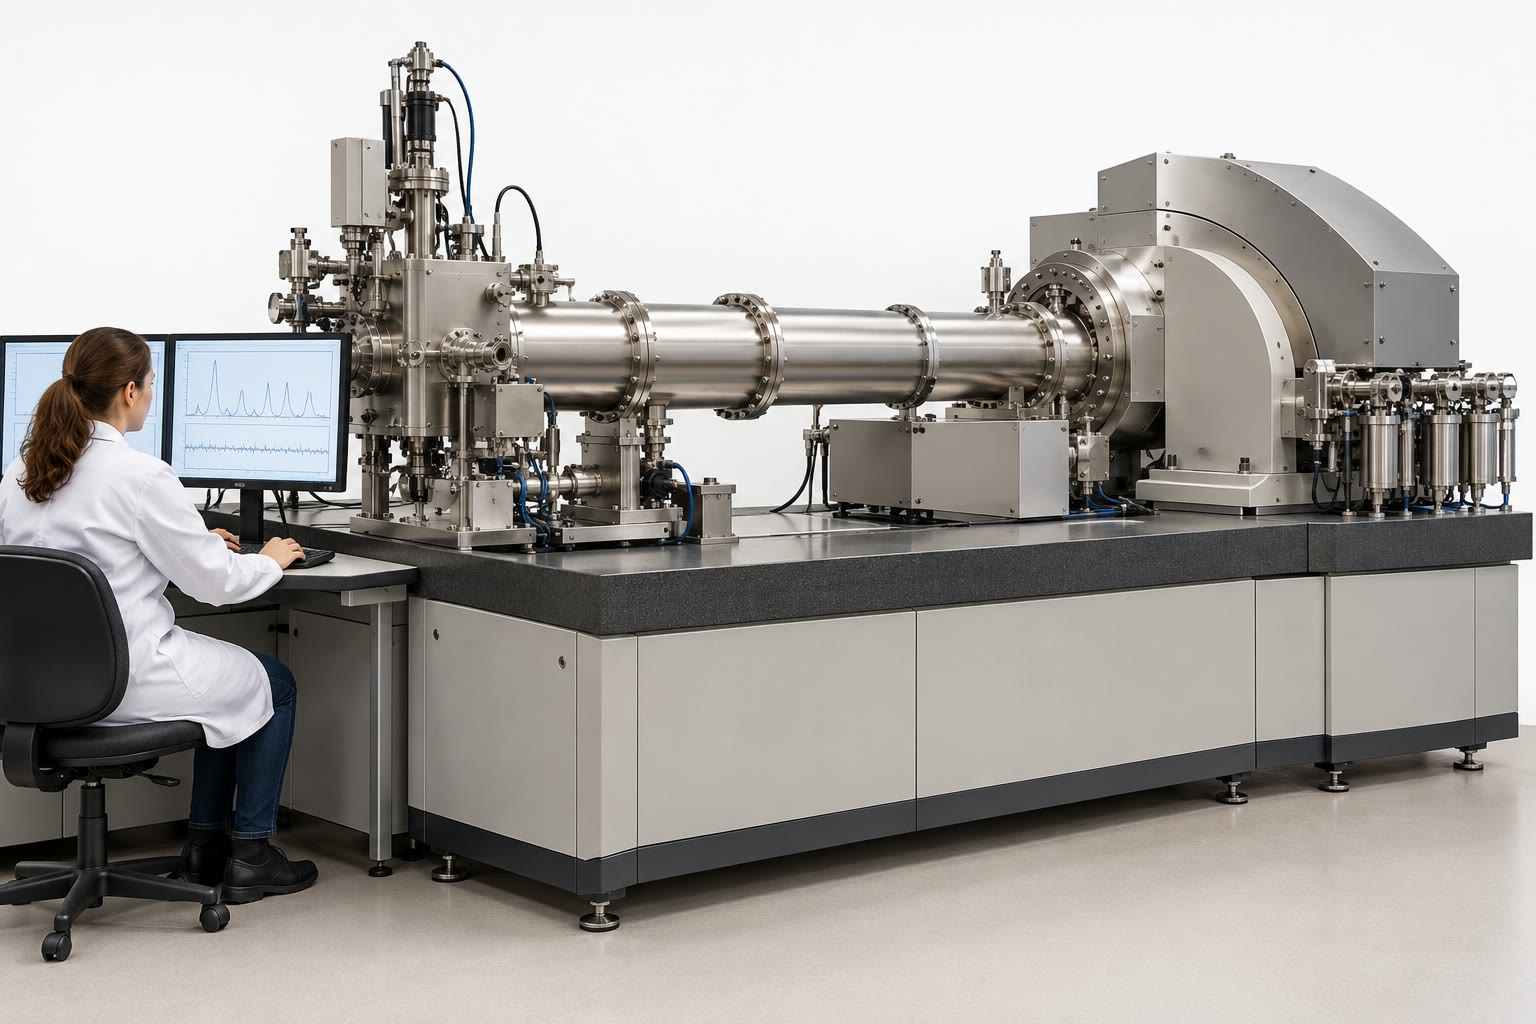
\includegraphics[width=\linewidth]{images/book4/ai/b2-isotope-lab.jpg}
\par\smallskip{\scriptsize Een multicollectormassaspectrometer in een
isotopenlaboratorium (door AI gegenereerde illustratie).}
\end{minipage}
\end{inthelab}
% ledger: white:chur

\section{Oefeningen}

\begin{exercise}[$\star$]\label{exo:b2:isotope-geochemistry:1}
Een basalt van Tristan da Cunha heeft $^{143}\mathrm{Nd}/^{144}\mathrm{Nd} = 0.51249$ en
een van Mangaia 0.51285. Bereken hun $\varepsilon_{\mathrm{Nd}}$ en die van de gemiddelde
MORB (0.513074). Welke bronnen hebben een hogere Sm/Nd gehad dan \omterm{def:b2:planet-formation-meteorites:chondrule}{chondrieten}?
\end{exercise}

\begin{exercise}[$\star$]\label{exo:b2:isotope-geochemistry:2}
De verhouding $^{18}\mathrm{O}/^{16}\mathrm{O}$ is \num{2.0052e-3} in \omterm{def:b2:isotope-geochemistry:standards}{VSMOW} en
\num{2.0672e-3} in \omterm{def:b2:isotope-geochemistry:standards}{VPDB}. Wat is de $\delta^{18}\mathrm{O}$ van \omterm{def:b2:isotope-geochemistry:standards}{VPDB} op de VSMOW-schaal?
Een calciet heeft $\delta^{18}\mathrm{O} = -2.0$ promille (\omterm{def:b2:isotope-geochemistry:standards}{VPDB}); bereken zijn verhouding
en zijn $\delta^{18}\mathrm{O}$ op de VSMOW-schaal.
\end{exercise}

\begin{exercise}[$\star$]\label{exo:b2:isotope-geochemistry:3}
Bereken de $^{143}\mathrm{Nd}/^{144}\mathrm{Nd}$ van CHUR \qty{1.0}{Ga} en
\qty{4.567}{Ga} geleden ($\lambda_{147} = \qty{6.524e-12}{\per\year}$,
$^{147}\mathrm{Sm}/^{144}\mathrm{Nd} = 0.1966$, vandaag 0.512638).
\end{exercise}

\begin{exercise}[$\star$]\label{exo:b2:isotope-geochemistry:4}
Een sneeuwmonster van een bergstation heeft $\delta^{18}\mathrm{O} = -18.0$ promille.
Welke $\delta\mathrm{D}$ voorspelt de \omterm{prop:b2:isotope-geochemistry:mwl}{meteorische waterlijn}? Een meerwater heeft
$\delta^{18}\mathrm{O} = -4.0$ en $\delta\mathrm{D} = -42$ promille: bereken zijn
deuteriumoverschot $d = \delta\mathrm{D} - 8\delta^{18}\mathrm{O}$, en zeg of het boven of
onder de lijn ligt.
\end{exercise}

\begin{exercise}[$\star\star$]\label{exo:b2:isotope-geochemistry:5}
Bereken $Q$ van de propositie over lineaire groei. Een graniet heeft Sm \qty{6.0}{ppm}
en Nd \qty{30}{ppm} (CI: 0.145 en \qty{0.457}{ppm}). Bereken zijn
$f_{\mathrm{Sm/Nd}}$, en de verandering van zijn $\varepsilon_{\mathrm{Nd}}$ over
\qty{500}{Myr}.
\end{exercise}

\begin{exercise}[$\star\star$]\label{exo:b2:isotope-geochemistry:6}
Een korst scheidde zich \qty{2.7}{Ga} geleden af van een mantel met
$\varepsilon_{\mathrm{Nd}} = +3.5$, met $f_{\mathrm{Sm/Nd}} = -0.45$. Schat haar
$\varepsilon_{\mathrm{Nd}}$ van vandaag met de propositie over lineaire groei. De exacte
berekening geeft $-27.3$; hoeveel wijkt de benadering af, en waarom is ze
te hoog of te laag?
\end{exercise}

\begin{exercise}[$\star\star$]\label{exo:b2:isotope-geochemistry:7}
Een basaltisch magma (Sr \qty{130}{ppm}, $^{87}\mathrm{Sr}/^{86}\mathrm{Sr} = 0.7030$)
assimileert een graniet (Sr \qty{320}{ppm}, 0.7200). Bereken de
$^{87}\mathrm{Sr}/^{86}\mathrm{Sr}$ van mengsels met 5, 10 en 20 procent graniet.
Toon aan dat $^{87}\mathrm{Sr}/^{86}\mathrm{Sr}$ een rechte lijn is tegen $1/\mathrm{Sr}$
en geef de helling en het snijpunt.
\end{exercise}

\begin{exercise}[$\star\star$]\label{exo:b2:isotope-geochemistry:8}
Bereken met de fractioneringsfactoren vloeistof--damp 1.0098 ($^{18}$O) en 1.084 (D) bij
\qty{20}{\degreeCelsius} de $\delta^{18}\mathrm{O}$ en $\delta\mathrm{D}$ van een
damp in evenwicht met oceaanwater (0, 0), en de helling
$\delta\mathrm{D}/\delta^{18}\mathrm{O}$ van de lijn van het water naar de damp. Herhaal
bij \qty{0}{\degreeCelsius} (1.0117 en 1.111). Vergelijk met de \omterm{prop:b2:isotope-geochemistry:mwl}{meteorische waterlijn}.
\end{exercise}

\begin{exercise}[$\star\star$]\label{exo:b2:isotope-geochemistry:9}
De continentale korst is 0.51 procent van de massa van de silicaataarde en bevat
gemiddeld \qty{27}{ppm} Nd tegen \qty{1.25}{ppm} voor de silicaataarde. Neem
voor de $\varepsilon_{\mathrm{Nd}}$ van de korst $-15$ en voor die van de silicaataarde 0. Welk
aandeel van het neodymium bevat de korst? Als de rest van de mantel uniform was,
welke $\varepsilon_{\mathrm{Nd}}$ zou die dan hebben? Welk aandeel van het neodymium moet een
verarmd reservoir op $+8.5$ bevatten als de rest van de mantel chondritisch is?
\end{exercise}

\begin{exercise}[$\star\star\star$]\label{exo:b2:isotope-geochemistry:10}
Toon aan dat in de propositie over lineaire groei de verwaarloosde termen een relatieve
grootte van ongeveer $\lambda t/2$ hebben. Hoe groot is dit over de ouderdom van de aarde, en hoe
groot is de fout die het veroorzaakt in $\varepsilon_{\mathrm{Nd}}$ voor $f = -0.45$ over
\qty{2.7}{Ga}?
\end{exercise}

\begin{exercise}[$\star\star\star$]\label{exo:b2:isotope-geochemistry:11}
Twee componenten hebben Sr/Nd-verhoudingen van 13.3 (A) en 5.0 (B). Zoek met het bewijs van de
\omterm{prop:b2:isotope-geochemistry:mixing}{menghyperbool} het aandeel $s'$ van het strontium uit A in een mengsel waarin A
een aandeel $s = 0.5$ van het neodymium levert. Voor welke waarde van $s$ verschillen de twee
aandelen het meest?
\end{exercise}

\begin{exercise}[$\star\star\star$]\label{exo:b2:isotope-geochemistry:12}
Een boxmodel geeft 2.3 tot 2.6 keer het huidige volume continentale korst,
\qty{7.2e9}{km^3}, gevormd sinds de vorming van de aarde \qty{4.5}{Ga} geleden, en 1.3 tot 1.6
keer vernietigd. Bereken de gemiddelde snelheden van vorming en vernietiging in
\unit{km^3} per jaar. Vergelijk ze met de huidige snelheden bij subductiezones,
\qty{2.7}{km^3} per jaar toegevoegd en \qty{3.2}{km^3} per jaar verwijderd.
\end{exercise}

\section{Probleem: Drie eilanden, drie mantels}

\begin{problem}[{Weekendprobleem --- de lava's van drie eilanden op de
mantelreeks plaatsen, een mengsel van een derde component scheiden, en het
gerecyclede sediment dateren}]
\label{pb:b2:isotope-geochemistry:1}
Drie vulkanische eilanden van een denkbeeldige oceaan, Kora, Vel en Asha, produceren basalten
met de isotopenverhoudingen hieronder. Een geochemicus modelleert hun bronnen met twee
componenten: een \omterm{def:b2:isotope-geochemistry:reservoirs}{verarmde mantel} zoals de bron van MORB (Sr \qty{10}{ppm}, Nd
\qty{0.75}{ppm}, $^{87}\mathrm{Sr}/^{86}\mathrm{Sr} = 0.70282$,
$^{143}\mathrm{Nd}/^{144}\mathrm{Nd} = 0.51307$) en een oud sediment dat door subductie naar de
mantel is teruggekeerd (Sr \qty{200}{ppm}, Nd \qty{40}{ppm}, $0.72000$, $0.51141$;
$^{147}\mathrm{Sm}/^{144}\mathrm{Nd} = 0.110$, $^{87}\mathrm{Rb}/^{86}\mathrm{Sr} = 0.50$).
Kora: $0.70410$, $0.51278$; Vel: $0.70618$, $0.51242$; Asha: $0.70290$, $0.51288$
($^{87}\mathrm{Sr}/^{86}\mathrm{Sr}$, $^{143}\mathrm{Nd}/^{144}\mathrm{Nd}$). CHUR vandaag:
$^{143}\mathrm{Nd}/^{144}\mathrm{Nd} = 0.512638$, $^{147}\mathrm{Sm}/^{144}\mathrm{Nd} =
0.1966$; $\lambda_{147} = \qty{6.524e-12}{\per\year}$, $\lambda_{87} =
\qty{1.3972e-11}{\per\year}$.

\medskip\noindent\textbf{Deel I --- De eilanden plaatsen.}
\begin{enumerate}
\item Bereken $\varepsilon_{\mathrm{Nd}}$ van de twee componenten.
\item Bereken $\varepsilon_{\mathrm{Nd}}$ van de drie eilanden.
\item Plaats de vijf samenstellingen in een Sr--$\varepsilon_{\mathrm{Nd}}$-diagram. Welke
eilanden liggen aan de verrijkte kant van CHUR?
\item Asha heeft bijna de strontiumverhouding van de \omterm{def:b2:isotope-geochemistry:reservoirs}{verarmde mantel} maar een veel lagere
$\varepsilon_{\mathrm{Nd}}$. Waar ligt het ten opzichte van de mantelreeks, en op welke
eilandgroep van het hoofdstuk lijkt het?
\item Waarom mogen de isotopenverhoudingen van de lava's als die van hun bronnen worden genomen,
hoewel de lava's een heel andere Sm/Nd en Rb/Sr hebben dan hun bronnen?
\item Een lava van Kora met $^{147}\mathrm{Sm}/^{144}\mathrm{Nd} = 0.12$ is \qty{1}{Myr} oud.
Met hoeveel is haar $^{143}\mathrm{Nd}/^{144}\mathrm{Nd}$ sinds de eruptie gegroeid, in
epsiloneenheden? Doet dit ertoe?
\end{enumerate}

\noindent\textbf{Deel II --- De twee componenten mengen.}
\begin{enumerate}[resume]
\item Schrijf de Nd-concentratie en de $^{143}\mathrm{Nd}/^{144}\mathrm{Nd}$ van een
mengsel met een massafractie $f$ sediment.
\item Bereken $\varepsilon_{\mathrm{Nd}}$ van mengsels met $f = 0.5$, 1, 2 en 5
procent.
\item Bereken $^{87}\mathrm{Sr}/^{86}\mathrm{Sr}$ van dezelfde mengsels.
\item Toon aan dat de $^{87}\mathrm{Sr}/^{86}\mathrm{Sr}$ van de mengsels een rechte
lijn is tegen $1/\mathrm{Sr}$, en geef de helling.
\item Bereken $K = (\mathrm{Sr}/\mathrm{Nd})_{\text{mantel}}/(\mathrm{Sr}/\mathrm{Nd})_{\text{sediment}}$.
Welke verhouding, die van Sr of die van Nd, beweegt sneller naar het sediment als $f$ groeit?
\item Hoeveel keer is het sediment rijker dan de mantel aan Nd, en aan Sr?
Leg met deze getallen uit waarom één procent sediment
$\varepsilon_{\mathrm{Nd}}$ met ongeveer 11 eenheden verschuift.
\item Welk aandeel van het neodymium van een mengsel met $f = 1$ procent komt van het
sediment?
\end{enumerate}

\noindent\textbf{Deel III --- Hoeveel sediment?}
\begin{enumerate}[resume]
\item Los de Nd-mengvergelijking op naar $f$, gegeven de verhouding $R$ van het mengsel.
\item Bereken $f$ voor Kora uit zijn neodymium.
\item Bereken $f$ voor Kora uit zijn strontium. Komen de twee overeen?
\item Bereken $f$ voor Vel uit zijn neodymium en uit zijn strontium.
\item Bereken $f$ voor Asha uit zijn neodymium, en de strontiumverhouding die deze $f$
voorspelt. Vergelijk met de gemeten waarde: wat volgt daaruit voor de bron van
Asha?
\item Stel uit het hoofdstuk een derde component voor Asha voor, en de
verhoudingen moeder--dochter die die component moet hebben gehad.
\end{enumerate}

\noindent\textbf{Deel IV --- De ouderdom van het sediment.}
\begin{enumerate}[resume]
\item Het sediment werd \qty{2.0}{Ga} geleden gesubduceerd en is sindsdien gesloten.
Bereken zijn $^{143}\mathrm{Nd}/^{144}\mathrm{Nd}$, die van CHUR en zijn
$\varepsilon_{\mathrm{Nd}}$ op dat moment.
\item Herhaal de berekening met de propositie over lineaire groei.
\item Bereken de $^{87}\mathrm{Sr}/^{86}\mathrm{Sr}$ van het sediment \qty{2.0}{Ga} geleden.
\item \qty{2.0}{Ga} geleden had de korst van de $\varepsilon_{\mathrm{Nd}}$-figuur
$\varepsilon_{\mathrm{Nd}} \approx -4.7$. Is de waarde van het sediment bij de subductie verenigbaar
met een herkomst door erosie van zo'n jonge continentale korst?
\item Geef de massafractie gerecycled sediment in de bron van het meest
verrijkte eiland, het kerngetal van dit probleem.
\end{enumerate}
\end{problem}
% ledger: white:chur, villa20:sm147, villa22:rb87, gale13:isotopes
